% Options for packages loaded elsewhere
\PassOptionsToPackage{unicode}{hyperref}
\PassOptionsToPackage{hyphens}{url}
%
\documentclass[
]{article}
\title{SemiMech Covid Forecasting}
\author{}
\date{\vspace{-2.5em}}

\usepackage{amsmath,amssymb}
\usepackage{lmodern}
\usepackage{iftex}
\ifPDFTeX
  \usepackage[T1]{fontenc}
  \usepackage[utf8]{inputenc}
  \usepackage{textcomp} % provide euro and other symbols
\else % if luatex or xetex
  \usepackage{unicode-math}
  \defaultfontfeatures{Scale=MatchLowercase}
  \defaultfontfeatures[\rmfamily]{Ligatures=TeX,Scale=1}
\fi
% Use upquote if available, for straight quotes in verbatim environments
\IfFileExists{upquote.sty}{\usepackage{upquote}}{}
\IfFileExists{microtype.sty}{% use microtype if available
  \usepackage[]{microtype}
  \UseMicrotypeSet[protrusion]{basicmath} % disable protrusion for tt fonts
}{}
\makeatletter
\@ifundefined{KOMAClassName}{% if non-KOMA class
  \IfFileExists{parskip.sty}{%
    \usepackage{parskip}
  }{% else
    \setlength{\parindent}{0pt}
    \setlength{\parskip}{6pt plus 2pt minus 1pt}}
}{% if KOMA class
  \KOMAoptions{parskip=half}}
\makeatother
\usepackage{xcolor}
\IfFileExists{xurl.sty}{\usepackage{xurl}}{} % add URL line breaks if available
\IfFileExists{bookmark.sty}{\usepackage{bookmark}}{\usepackage{hyperref}}
\hypersetup{
  pdftitle={SemiMech Covid Forecasting},
  hidelinks,
  pdfcreator={LaTeX via pandoc}}
\urlstyle{same} % disable monospaced font for URLs
\usepackage[margin=1in]{geometry}
\usepackage{color}
\usepackage{fancyvrb}
\newcommand{\VerbBar}{|}
\newcommand{\VERB}{\Verb[commandchars=\\\{\}]}
\DefineVerbatimEnvironment{Highlighting}{Verbatim}{commandchars=\\\{\}}
% Add ',fontsize=\small' for more characters per line
\usepackage{framed}
\definecolor{shadecolor}{RGB}{248,248,248}
\newenvironment{Shaded}{\begin{snugshade}}{\end{snugshade}}
\newcommand{\AlertTok}[1]{\textcolor[rgb]{0.94,0.16,0.16}{#1}}
\newcommand{\AnnotationTok}[1]{\textcolor[rgb]{0.56,0.35,0.01}{\textbf{\textit{#1}}}}
\newcommand{\AttributeTok}[1]{\textcolor[rgb]{0.77,0.63,0.00}{#1}}
\newcommand{\BaseNTok}[1]{\textcolor[rgb]{0.00,0.00,0.81}{#1}}
\newcommand{\BuiltInTok}[1]{#1}
\newcommand{\CharTok}[1]{\textcolor[rgb]{0.31,0.60,0.02}{#1}}
\newcommand{\CommentTok}[1]{\textcolor[rgb]{0.56,0.35,0.01}{\textit{#1}}}
\newcommand{\CommentVarTok}[1]{\textcolor[rgb]{0.56,0.35,0.01}{\textbf{\textit{#1}}}}
\newcommand{\ConstantTok}[1]{\textcolor[rgb]{0.00,0.00,0.00}{#1}}
\newcommand{\ControlFlowTok}[1]{\textcolor[rgb]{0.13,0.29,0.53}{\textbf{#1}}}
\newcommand{\DataTypeTok}[1]{\textcolor[rgb]{0.13,0.29,0.53}{#1}}
\newcommand{\DecValTok}[1]{\textcolor[rgb]{0.00,0.00,0.81}{#1}}
\newcommand{\DocumentationTok}[1]{\textcolor[rgb]{0.56,0.35,0.01}{\textbf{\textit{#1}}}}
\newcommand{\ErrorTok}[1]{\textcolor[rgb]{0.64,0.00,0.00}{\textbf{#1}}}
\newcommand{\ExtensionTok}[1]{#1}
\newcommand{\FloatTok}[1]{\textcolor[rgb]{0.00,0.00,0.81}{#1}}
\newcommand{\FunctionTok}[1]{\textcolor[rgb]{0.00,0.00,0.00}{#1}}
\newcommand{\ImportTok}[1]{#1}
\newcommand{\InformationTok}[1]{\textcolor[rgb]{0.56,0.35,0.01}{\textbf{\textit{#1}}}}
\newcommand{\KeywordTok}[1]{\textcolor[rgb]{0.13,0.29,0.53}{\textbf{#1}}}
\newcommand{\NormalTok}[1]{#1}
\newcommand{\OperatorTok}[1]{\textcolor[rgb]{0.81,0.36,0.00}{\textbf{#1}}}
\newcommand{\OtherTok}[1]{\textcolor[rgb]{0.56,0.35,0.01}{#1}}
\newcommand{\PreprocessorTok}[1]{\textcolor[rgb]{0.56,0.35,0.01}{\textit{#1}}}
\newcommand{\RegionMarkerTok}[1]{#1}
\newcommand{\SpecialCharTok}[1]{\textcolor[rgb]{0.00,0.00,0.00}{#1}}
\newcommand{\SpecialStringTok}[1]{\textcolor[rgb]{0.31,0.60,0.02}{#1}}
\newcommand{\StringTok}[1]{\textcolor[rgb]{0.31,0.60,0.02}{#1}}
\newcommand{\VariableTok}[1]{\textcolor[rgb]{0.00,0.00,0.00}{#1}}
\newcommand{\VerbatimStringTok}[1]{\textcolor[rgb]{0.31,0.60,0.02}{#1}}
\newcommand{\WarningTok}[1]{\textcolor[rgb]{0.56,0.35,0.01}{\textbf{\textit{#1}}}}
\usepackage{graphicx}
\makeatletter
\def\maxwidth{\ifdim\Gin@nat@width>\linewidth\linewidth\else\Gin@nat@width\fi}
\def\maxheight{\ifdim\Gin@nat@height>\textheight\textheight\else\Gin@nat@height\fi}
\makeatother
% Scale images if necessary, so that they will not overflow the page
% margins by default, and it is still possible to overwrite the defaults
% using explicit options in \includegraphics[width, height, ...]{}
\setkeys{Gin}{width=\maxwidth,height=\maxheight,keepaspectratio}
% Set default figure placement to htbp
\makeatletter
\def\fps@figure{htbp}
\makeatother
\setlength{\emergencystretch}{3em} % prevent overfull lines
\providecommand{\tightlist}{%
  \setlength{\itemsep}{0pt}\setlength{\parskip}{0pt}}
\setcounter{secnumdepth}{-\maxdimen} % remove section numbering
\ifLuaTeX
  \usepackage{selnolig}  % disable illegal ligatures
\fi

\begin{document}
\maketitle

\hypertarget{introduction}{%
\subsection{Introduction}\label{introduction}}

Please see influenza vignette for description

\hypertarget{application-to-covid-19-hospitalization-forecasting}{%
\subsection{Application to COVID-19 hospitalization
forecasting}\label{application-to-covid-19-hospitalization-forecasting}}

First, we will download the data we need for forecasting influenza
hospitalizations

\begin{Shaded}
\begin{Highlighting}[]
\FunctionTok{library}\NormalTok{(stringr)}
\CommentTok{\#setwd("../")}
\FunctionTok{source}\NormalTok{(}\StringTok{\textquotesingle{}R/get\_hhs.R\textquotesingle{}}\NormalTok{)}
\end{Highlighting}
\end{Shaded}

\begin{verbatim}
## 
## Attaching package: 'dplyr'
\end{verbatim}

\begin{verbatim}
## The following objects are masked from 'package:stats':
## 
##     filter, lag
\end{verbatim}

\begin{verbatim}
## The following objects are masked from 'package:base':
## 
##     intersect, setdiff, setequal, union
\end{verbatim}

\begin{Shaded}
\begin{Highlighting}[]
\NormalTok{hhs }\OtherTok{\textless{}{-}} \FunctionTok{get\_hhs}\NormalTok{()}
\end{Highlighting}
\end{Shaded}

\begin{verbatim}
## Loading required package: RSocrata
\end{verbatim}

\begin{verbatim}
## Loading required package: readr
\end{verbatim}

\begin{verbatim}
## Warning in read.socrata("https://healthdata.gov/resource/g62h-syeh.csv", : Dates
## and currency fields will be converted to character
\end{verbatim}

\begin{verbatim}
## Rows: 51 Columns: 4
\end{verbatim}

\begin{verbatim}
## -- Column specification --------------------------------------------------------
## Delimiter: ","
## chr (3): FIPS, Name, Abbreviation
## dbl (1): Alphacount
## 
## i Use `spec()` to retrieve the full column specification for this data.
## i Specify the column types or set `show_col_types = FALSE` to quiet this message.
## Rows: 56 Columns: 2
## -- Column specification --------------------------------------------------------
## Delimiter: ","
## chr (1): location
## dbl (1): Pop_Est_2019
## 
## i Use `spec()` to retrieve the full column specification for this data.
## i Specify the column types or set `show_col_types = FALSE` to quiet this message.
## Joining, by = "state"
## Joining, by = "state_full"
\end{verbatim}

Let's plot Texas (TX) as our example state.

\begin{Shaded}
\begin{Highlighting}[]
\FunctionTok{library}\NormalTok{(ggplot2)}
\FunctionTok{ggplot}\NormalTok{(hhs[hhs}\SpecialCharTok{$}\NormalTok{state }\SpecialCharTok{==} \StringTok{"TX"}\NormalTok{,],}\FunctionTok{aes}\NormalTok{(}\AttributeTok{x=}\NormalTok{date,}\AttributeTok{y=}\NormalTok{total\_adult\_patients\_hospitalized\_confirmed\_covid))}\SpecialCharTok{+} \FunctionTok{geom\_line}\NormalTok{()}
\end{Highlighting}
\end{Shaded}

\begin{verbatim}
## Warning: Removed 196 row(s) containing missing values (geom_path).
\end{verbatim}

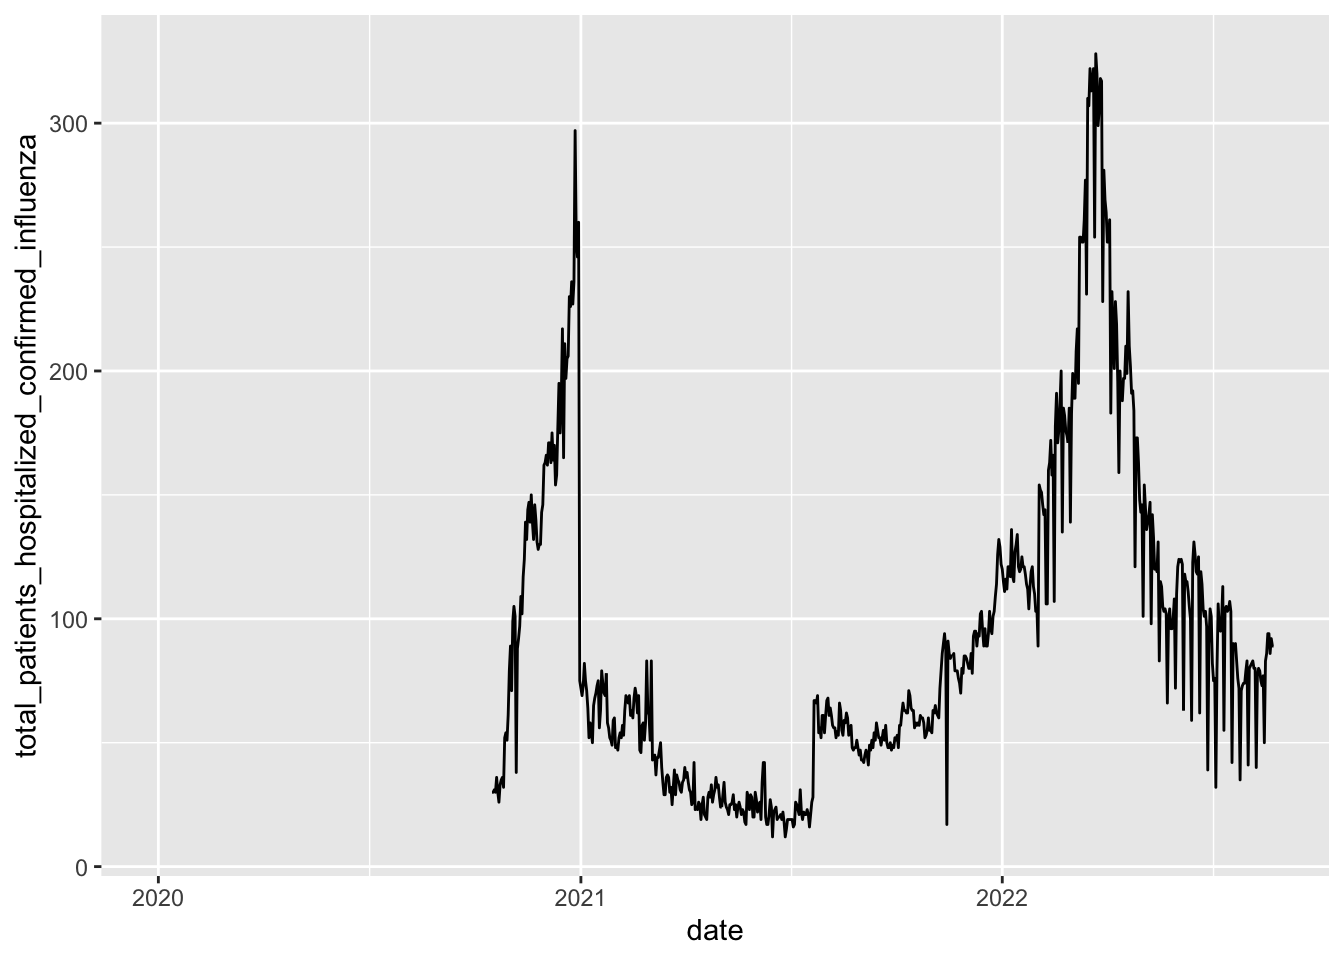
\includegraphics{covid_hosp_vignette_files/figure-latex/unnamed-chunk-2-1.pdf}

Unlike influenza hospitalizations, COVID-19 does not have a set
seasonality. To handle this we need to extract the ``waves'' that occur
in COVID-19 data. To do this, we first smooth the time series and
extract the derivative.

\begin{Shaded}
\begin{Highlighting}[]
\NormalTok{tx\_hosps }\OtherTok{\textless{}{-}}\NormalTok{ hhs[hhs}\SpecialCharTok{$}\NormalTok{state }\SpecialCharTok{==} \StringTok{"TX"}\NormalTok{,]}\SpecialCharTok{$}\NormalTok{total\_adult\_patients\_hospitalized\_confirmed\_covid}
\NormalTok{smoothed\_deriv }\OtherTok{\textless{}{-}} \FunctionTok{c}\NormalTok{(}\DecValTok{0}\NormalTok{,}\FunctionTok{diff}\NormalTok{(}\FunctionTok{lowess}\NormalTok{(tx\_hosps}\SpecialCharTok{/}\FunctionTok{max}\NormalTok{(tx\_hosps,}\AttributeTok{na.rm=}\NormalTok{T),}\AttributeTok{f=}\NormalTok{.}\DecValTok{1}\NormalTok{)}\SpecialCharTok{$}\NormalTok{y))}
\FunctionTok{plot}\NormalTok{(tx\_hosps}\SpecialCharTok{/}\FunctionTok{max}\NormalTok{(tx\_hosps,}\AttributeTok{na.rm=}\NormalTok{T),}\AttributeTok{type=}\StringTok{\textquotesingle{}l\textquotesingle{}}\NormalTok{,}\AttributeTok{ylim=}\FunctionTok{c}\NormalTok{(}\SpecialCharTok{{-}}\DecValTok{1}\NormalTok{,}\DecValTok{1}\NormalTok{))}
\FunctionTok{lines}\NormalTok{(}\DecValTok{10}\SpecialCharTok{*}\NormalTok{smoothed\_deriv,}\AttributeTok{type=}\StringTok{\textquotesingle{}l\textquotesingle{}}\NormalTok{)}
\FunctionTok{abline}\NormalTok{(}\AttributeTok{h=}\DecValTok{0}\NormalTok{,}\AttributeTok{col=}\StringTok{\textquotesingle{}red\textquotesingle{}}\NormalTok{)}
\end{Highlighting}
\end{Shaded}

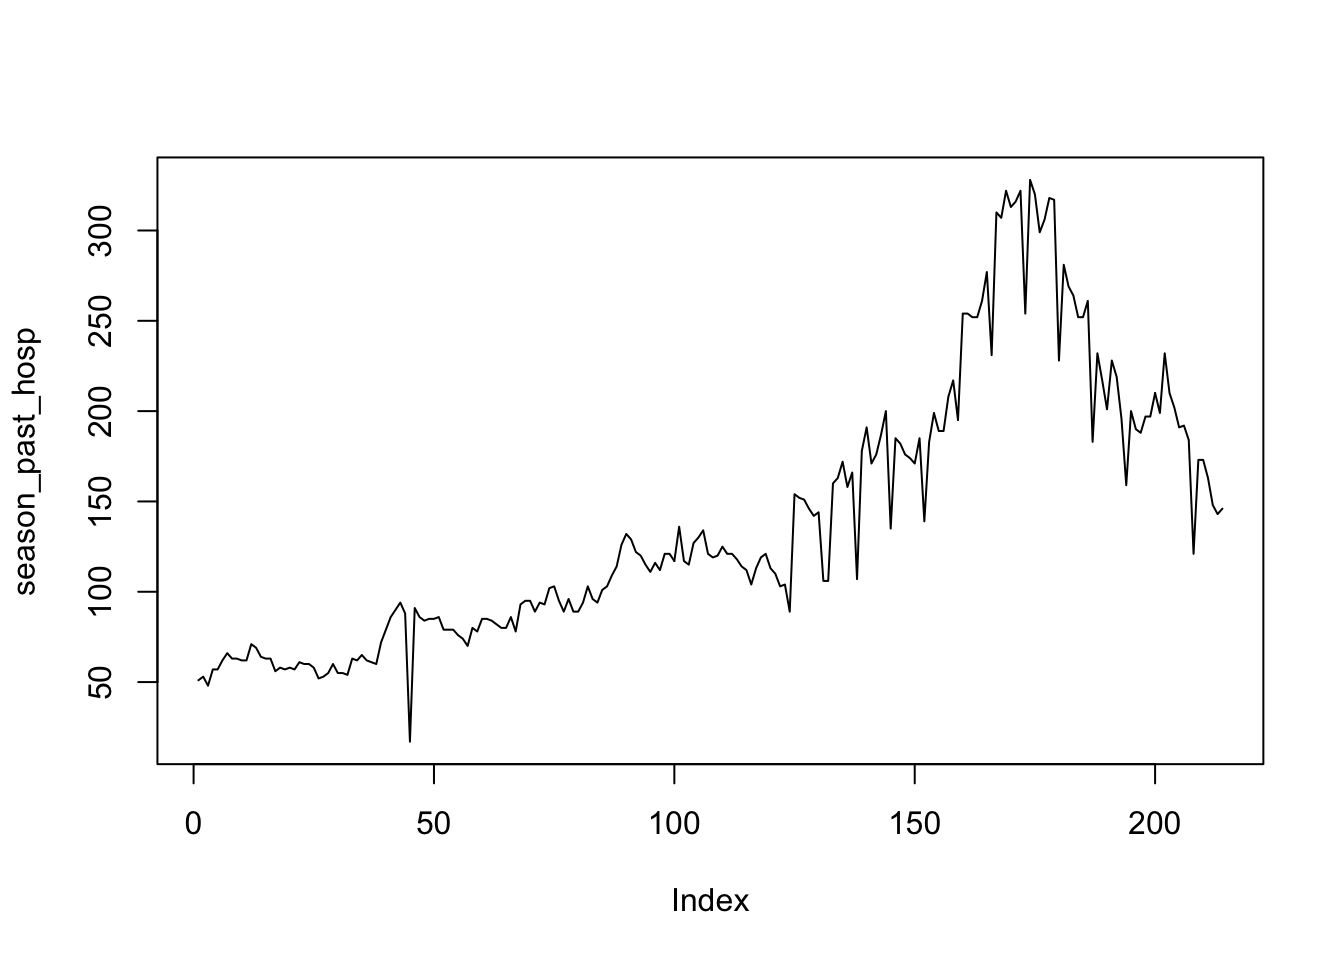
\includegraphics{covid_hosp_vignette_files/figure-latex/unnamed-chunk-3-1.pdf}

As we can see from the plot, the points at which the derivative goes
from negative to positive are good indicators of the beginning of a
wave. Let's now extract the waves.

\begin{Shaded}
\begin{Highlighting}[]
\NormalTok{wave\_starts }\OtherTok{\textless{}{-}} \FunctionTok{c}\NormalTok{()}

\ControlFlowTok{for}\NormalTok{ (t }\ControlFlowTok{in} \DecValTok{2}\SpecialCharTok{:}\FunctionTok{length}\NormalTok{(smoothed\_deriv))\{}
  \ControlFlowTok{if}\NormalTok{ (}\SpecialCharTok{!}\FunctionTok{is.na}\NormalTok{(smoothed\_deriv[t}\DecValTok{{-}1}\NormalTok{]) }\SpecialCharTok{\&} \SpecialCharTok{!}\FunctionTok{is.na}\NormalTok{(smoothed\_deriv[t]))\{}
    \ControlFlowTok{if}\NormalTok{ (smoothed\_deriv[t}\DecValTok{{-}1}\NormalTok{] }\SpecialCharTok{\textless{}} \DecValTok{0} \SpecialCharTok{\&}\NormalTok{ smoothed\_deriv[t] }\SpecialCharTok{\textgreater{}}\DecValTok{0}\NormalTok{)\{}
\NormalTok{      wave\_starts }\OtherTok{\textless{}{-}}\FunctionTok{c}\NormalTok{(wave\_starts,t)}
\NormalTok{    \}}
\NormalTok{  \}}
\NormalTok{\}}

\FunctionTok{print}\NormalTok{ (wave\_starts)}
\end{Highlighting}
\end{Shaded}

\begin{verbatim}
## [1] 533 695 848
\end{verbatim}

Lets add the wave starts to the plot we generated above.

\begin{Shaded}
\begin{Highlighting}[]
\FunctionTok{plot}\NormalTok{(tx\_hosps}\SpecialCharTok{/}\FunctionTok{max}\NormalTok{(tx\_hosps,}\AttributeTok{na.rm=}\NormalTok{T),}\AttributeTok{type=}\StringTok{\textquotesingle{}l\textquotesingle{}}\NormalTok{,}\AttributeTok{ylim=}\FunctionTok{c}\NormalTok{(}\SpecialCharTok{{-}}\DecValTok{1}\NormalTok{,}\DecValTok{1}\NormalTok{))}
\FunctionTok{lines}\NormalTok{(}\DecValTok{10}\SpecialCharTok{*}\NormalTok{smoothed\_deriv,}\AttributeTok{type=}\StringTok{\textquotesingle{}l\textquotesingle{}}\NormalTok{)}
\FunctionTok{abline}\NormalTok{(}\AttributeTok{h=}\DecValTok{0}\NormalTok{,}\AttributeTok{col=}\StringTok{\textquotesingle{}red\textquotesingle{}}\NormalTok{)}

\ControlFlowTok{for}\NormalTok{ (ws }\ControlFlowTok{in}\NormalTok{ wave\_starts)\{}
  \FunctionTok{abline}\NormalTok{(}\AttributeTok{v=}\NormalTok{ws,}\AttributeTok{col=}\StringTok{\textquotesingle{}blue\textquotesingle{}}\NormalTok{)}
\NormalTok{\}}
\end{Highlighting}
\end{Shaded}

\includegraphics{covid_hosp_vignette_files/figure-latex/unnamed-chunk-5-1.pdf}
We can see that the algorithm nicely identified two waves, except for
the start of the wave, which we will handle later.

Let's first extract the existing waves and plot them hierarchically.

\begin{Shaded}
\begin{Highlighting}[]
\NormalTok{wave\_matrix }\OtherTok{\textless{}{-}}\FunctionTok{matrix}\NormalTok{(}\ConstantTok{NA}\NormalTok{,}\AttributeTok{nrow=}\FunctionTok{length}\NormalTok{(wave\_starts)}\SpecialCharTok{{-}}\DecValTok{1}\NormalTok{,}\AttributeTok{ncol=}\DecValTok{1000}\NormalTok{)}

\ControlFlowTok{for}\NormalTok{ (wave\_start }\ControlFlowTok{in} \DecValTok{2}\SpecialCharTok{:}\FunctionTok{length}\NormalTok{(wave\_starts))\{}
\NormalTok{  to\_replace }\OtherTok{\textless{}{-}}\NormalTok{ tx\_hosps[wave\_starts[wave\_start}\DecValTok{{-}1}\NormalTok{]}\SpecialCharTok{:}\NormalTok{wave\_starts[wave\_start]]}
  \ControlFlowTok{while}\NormalTok{ (}\FunctionTok{length}\NormalTok{(to\_replace) }\SpecialCharTok{\textless{}} \DecValTok{1000}\NormalTok{)\{}
\NormalTok{    to\_replace }\OtherTok{\textless{}{-}} \FunctionTok{c}\NormalTok{(to\_replace,}\ConstantTok{NA}\NormalTok{)}
\NormalTok{  \}}
\NormalTok{  wave\_matrix[wave\_start}\DecValTok{{-}1}\NormalTok{,] }\OtherTok{\textless{}{-}}\NormalTok{ to\_replace}
\NormalTok{\}}


\NormalTok{NAindex }\OtherTok{\textless{}{-}}\ControlFlowTok{function}\NormalTok{(z)\{ }\FunctionTok{min}\NormalTok{(}\FunctionTok{which}\NormalTok{(}\FunctionTok{is.na}\NormalTok{(z)))\}}

\NormalTok{longest\_wave\_length }\OtherTok{\textless{}{-}} \FunctionTok{max}\NormalTok{(}\FunctionTok{apply}\NormalTok{(wave\_matrix,}\DecValTok{1}\NormalTok{,NAindex))}

\NormalTok{wave\_matrix }\OtherTok{\textless{}{-}}\NormalTok{ wave\_matrix[,}\DecValTok{1}\SpecialCharTok{:}\NormalTok{longest\_wave\_length]}

\FunctionTok{plot}\NormalTok{(}\DecValTok{0}\NormalTok{,}\AttributeTok{xlim=}\FunctionTok{c}\NormalTok{(}\DecValTok{0}\NormalTok{,longest\_wave\_length),}\AttributeTok{ylim=}\FunctionTok{c}\NormalTok{(}\DecValTok{0}\NormalTok{,}\DecValTok{20000}\NormalTok{))}
\ControlFlowTok{for}\NormalTok{ (row }\ControlFlowTok{in} \DecValTok{1}\SpecialCharTok{:}\FunctionTok{nrow}\NormalTok{(wave\_matrix))\{}
  \FunctionTok{lines}\NormalTok{(wave\_matrix[row,])}
\NormalTok{\}}
\end{Highlighting}
\end{Shaded}

\includegraphics{covid_hosp_vignette_files/figure-latex/unnamed-chunk-6-1.pdf}

These are the historical waves we can use for training. We also need the
current wave to fit.

\begin{Shaded}
\begin{Highlighting}[]
\NormalTok{current\_wave }\OtherTok{\textless{}{-}}\NormalTok{ tx\_hosps[wave\_starts[}\FunctionTok{length}\NormalTok{(wave\_starts)]}\SpecialCharTok{:}\FunctionTok{length}\NormalTok{(tx\_hosps)]}
\FunctionTok{plot}\NormalTok{(}\DecValTok{0}\NormalTok{,}\AttributeTok{xlim=}\FunctionTok{c}\NormalTok{(}\DecValTok{0}\NormalTok{,}\DecValTok{200}\NormalTok{),}\AttributeTok{ylim=}\FunctionTok{c}\NormalTok{(}\DecValTok{0}\NormalTok{,}\DecValTok{20000}\NormalTok{))}
\ControlFlowTok{for}\NormalTok{ (row }\ControlFlowTok{in} \DecValTok{1}\SpecialCharTok{:}\FunctionTok{nrow}\NormalTok{(wave\_matrix))\{}
  \FunctionTok{lines}\NormalTok{(wave\_matrix[row,])}
\NormalTok{\}}
\FunctionTok{lines}\NormalTok{(current\_wave,}\AttributeTok{col=}\StringTok{\textquotesingle{}red\textquotesingle{}}\NormalTok{)}
\end{Highlighting}
\end{Shaded}

\includegraphics{covid_hosp_vignette_files/figure-latex/unnamed-chunk-7-1.pdf}

\begin{Shaded}
\begin{Highlighting}[]
\FunctionTok{source}\NormalTok{(}\StringTok{\textquotesingle{}R/semimech2.R\textquotesingle{}}\NormalTok{)}
\end{Highlighting}
\end{Shaded}

\begin{verbatim}
## Loading required package: coda
\end{verbatim}

\begin{verbatim}
## Linked to JAGS 4.3.0
\end{verbatim}

\begin{verbatim}
## Loaded modules: basemod,bugs
\end{verbatim}

\begin{verbatim}
## 
## Attaching package: 'R2jags'
\end{verbatim}

\begin{verbatim}
## The following object is masked from 'package:coda':
## 
##     traceplot
\end{verbatim}

\begin{Shaded}
\begin{Highlighting}[]
\NormalTok{forecast }\OtherTok{\textless{}{-}} \FunctionTok{run\_semi\_mech}\NormalTok{(}\AttributeTok{season\_past\_matrix\_hosp =}\NormalTok{ wave\_matrix,}\AttributeTok{season\_current\_hosp =}\NormalTok{current\_wave )}
\end{Highlighting}
\end{Shaded}

\begin{verbatim}
## module glm loaded
\end{verbatim}

\begin{verbatim}
## Compiling model graph
##    Resolving undeclared variables
##    Allocating nodes
## Graph information:
##    Observed stochastic nodes: 435
##    Unobserved stochastic nodes: 535
##    Total graph size: 8898
## 
## Initializing model
\end{verbatim}

\includegraphics{covid_hosp_vignette_files/figure-latex/unnamed-chunk-8-1.pdf}

\begin{Shaded}
\begin{Highlighting}[]
\FunctionTok{plot}\NormalTok{(}\FunctionTok{colMeans}\NormalTok{(forecast))}
\end{Highlighting}
\end{Shaded}

\includegraphics{covid_hosp_vignette_files/figure-latex/unnamed-chunk-8-2.pdf}

Now we have a forecast object, lets make some plots.

\begin{Shaded}
\begin{Highlighting}[]
\NormalTok{forecast\_dates }\OtherTok{\textless{}{-}} \FunctionTok{seq}\NormalTok{(}\FunctionTok{as.Date}\NormalTok{(}\FunctionTok{tail}\NormalTok{(hhs}\SpecialCharTok{$}\NormalTok{date,}\DecValTok{1}\NormalTok{)),}\FunctionTok{as.Date}\NormalTok{(}\FunctionTok{tail}\NormalTok{(hhs}\SpecialCharTok{$}\NormalTok{date,}\DecValTok{1}\NormalTok{))}\SpecialCharTok{+}\DecValTok{29}\NormalTok{,}\AttributeTok{by=}\StringTok{"day"}\NormalTok{)}
\NormalTok{forecast\_df }\OtherTok{\textless{}{-}} \FunctionTok{data.frame}\NormalTok{(}\AttributeTok{date=}\NormalTok{forecast\_dates,}\AttributeTok{total\_adult\_patients\_hospitalized\_confirmed\_covid=}\FunctionTok{colMeans}\NormalTok{(forecast))}


\FunctionTok{ggplot}\NormalTok{(forecast\_df,}\FunctionTok{aes}\NormalTok{(}\AttributeTok{x=}\NormalTok{date,}\AttributeTok{y=}\NormalTok{total\_adult\_patients\_hospitalized\_confirmed\_covid,}\AttributeTok{col=}\StringTok{\textquotesingle{}forecast\textquotesingle{}}\NormalTok{)) }\SpecialCharTok{+} \FunctionTok{geom\_line}\NormalTok{() }\SpecialCharTok{+}
  \FunctionTok{geom\_line}\NormalTok{(}\AttributeTok{data=}\NormalTok{hhs[hhs}\SpecialCharTok{$}\NormalTok{state }\SpecialCharTok{==} \StringTok{"TX"}\NormalTok{  ,],}\FunctionTok{aes}\NormalTok{(}\AttributeTok{x=}\NormalTok{date,}\AttributeTok{y=}\NormalTok{total\_adult\_patients\_hospitalized\_confirmed\_covid,}\AttributeTok{col=}\StringTok{\textquotesingle{}Observed\textquotesingle{}}\NormalTok{))}
\end{Highlighting}
\end{Shaded}

\begin{verbatim}
## Warning: Removed 196 row(s) containing missing values (geom_path).
\end{verbatim}

\includegraphics{covid_hosp_vignette_files/figure-latex/unnamed-chunk-9-1.pdf}

\end{document}
